\section{Background Information \& Research}

\subsection{What is Fuzzy Logic?}
Fuzzy logic is a ``natural'' way of expressing uncertain or qualitative information \cite{albertos1998fuzzy}. It is a form of logic that deals with approximate reasoning, as opposed to fixed, exact values, like those found in classical logic (where we may only have properties being true, or false). Instead of these strict truth values, fuzzy logic systems have a range of truth, between 0 and 1. This makes fuzzy logic much better for handling and sorting data, and is an excellent choice for many control system applications, due to the way it mimics human control logic. Lotfi Zadeh, who formalised fuzzy logic in 1965, states that the key advantages of fuzzy logic are that it allows us to make rational decisions in environments of imprecision, uncertainty, and partiality of truth, and to perform a wide variety of physical and mental tasks, without any measurements or computations \cite{zadeh1999computing}.\\[2mm]
\noindent 
In a classical set, the membership, $\mu_A(x)$ of $x$, of a set, $A$, in universe, $X$, is defined:

\begin{center}
\vspace{-3mm}
$ 
\mu_A(x) = \left\lbrace
\begin{array}{ll}
1, & $iff x $\in$ A$      \\
0, & $iff x $\notin$ A$   \\
\end{array} \color{white}\right\rbrace $ 
\end{center}
\vspace{-2mm}
\noindent 
That is, the element is either in the set, or not. In a fuzzy set, however, we have grades of membership, which are real numbers in the interval, $\mu_A(x) \in [0,1]$. Every member of a set has a membership grade to that set, depicting how true the property represented by that set is, for the given member \cite{zadeh1965fuzzy}. The traditional syntax for representing members of a fuzzy set is given below (although a full working knowledge of fuzzy logic theory is not necessary for this project).
\vspace{-2mm}
\begin{center}
$A = \mu_A(x_1)/x_1 + ... + \mu_A(x_n)/x_n$
\end{center}
\vspace{-2mm}
The easiest way to observe the merits of fuzzy logic is to look at terms that we humans use in our everyday life, and attempt to map these as crisp functions. For instance, terms like ``hot'', ``cold'', ``tall'', and ``short'', are all terms that we understand very well, and use often. However, if we were asked to give \textit{exact} values for tallness, or shortness, we would not be able to do so. At what cut-off point would a person change from being considered short, to being considered tall? Fuzzy logic helps to alleviate these impossible choices, by having varying degrees of membership, for certain properties. The example in figure \ref{fig:fuzExample} shows this using three linguistic variables to describe the height of a person. Instead of at one point being either tall, short, or medium height, we, at all times, belong to all properties, to a differing degree. 

\begin{figure}[ht!]
\begin{center}
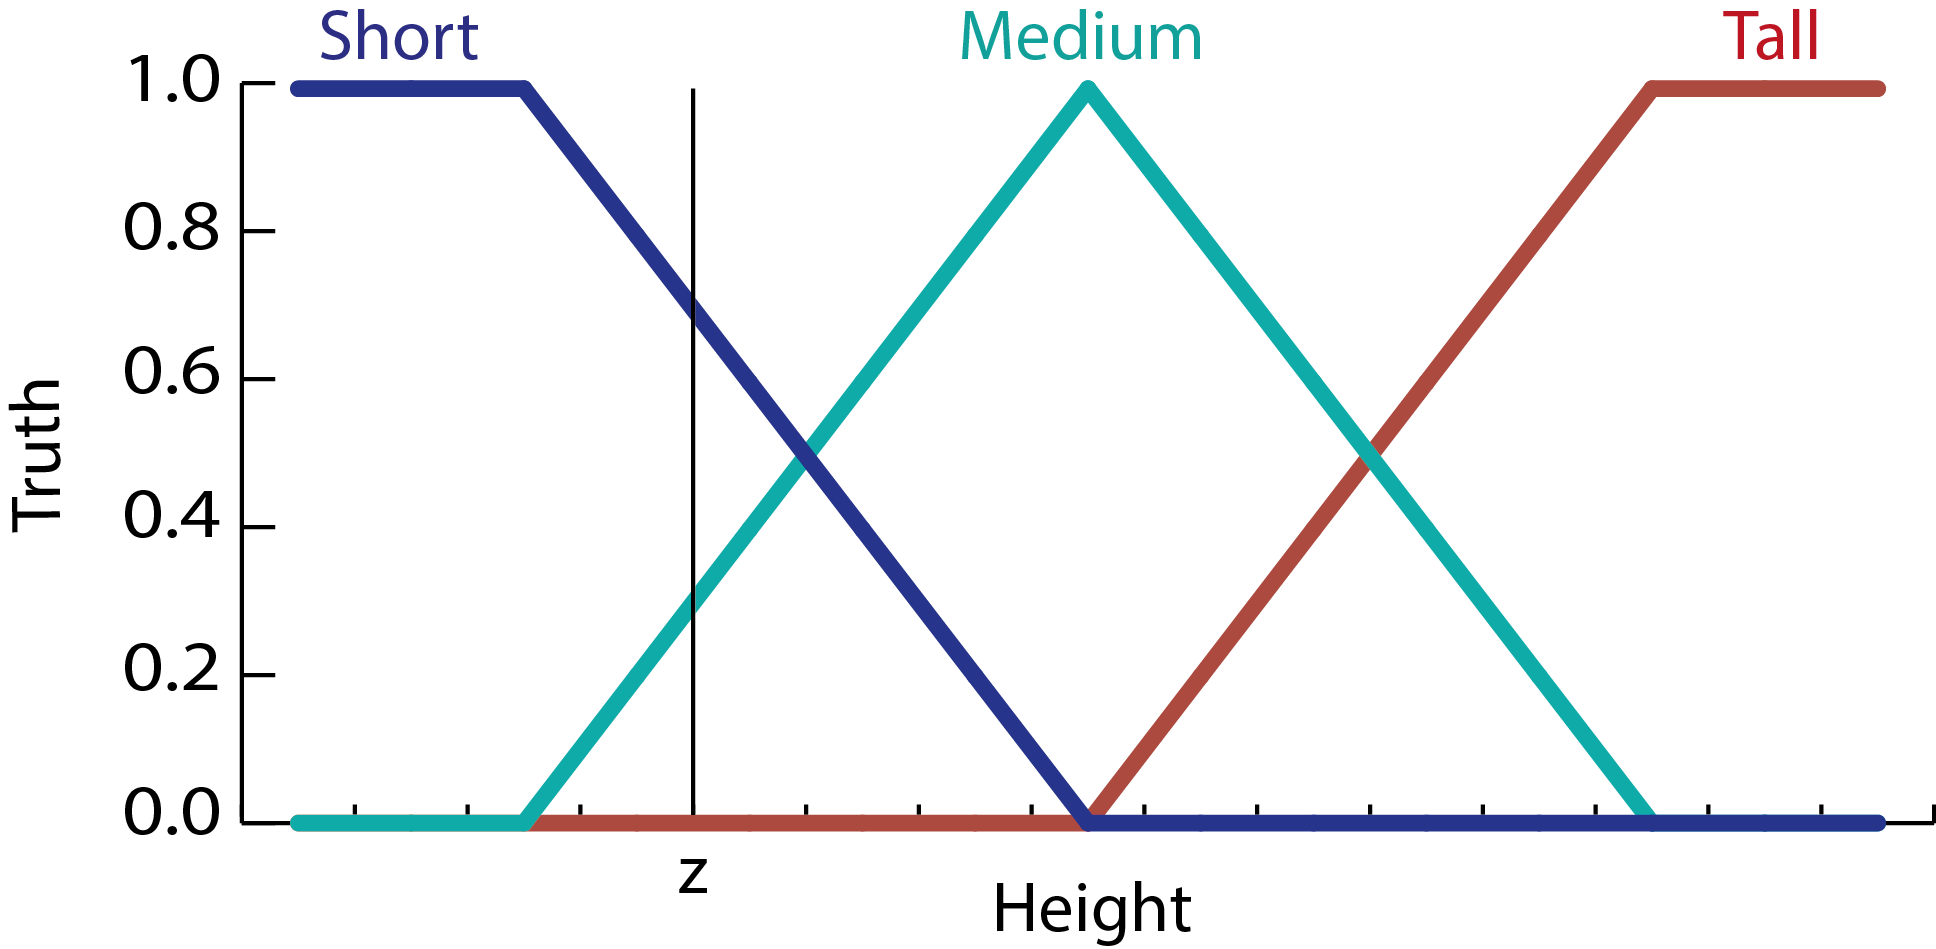
\includegraphics[width=0.6\textwidth]{images/fuzExample.png}
\end{center}
\vspace{-5mm}
\caption{A fuzzy set depicting ``height''}
\label{fig:fuzExample}
\end{figure}
\noindent
For instance, at the point labelled $z$, in the sets in figure \ref{fig:fuzExample}, the membership to the ``Short'' set is 0.7, the membership to the ``Medium'' set is 0.3, and membership to the ``Tall'' set, is 0.0. This is, naturally, much more precise than simply saying we are ``Short'', ``Medium'', or ``Tall''.

\subsection{Existing Systems}
\label{sec:existing-systems}

Fuzzy logic has been around for almost 50 years now, and, with the rising age of the computer, it would be alarming if no software systems for its usage were in circulation. Luckily, this is not the case, and there are many examples of software systems focusing on the use of fuzzy logic, of which many different approaches have been attempted, to varying degrees of success. In this section, a number of these software systems will be evaluated, to discern their positive and negative qualities, to help improve the design of the project presented in this report. 

\paragraph{MATLAB Fuzzy Toolbox}\ \\
The first system to be explored is MATLAB's fuzzy toolbox, an add-on for the MATLAB software suite, to work with fuzzy sets and systems. This toolbox provides everything required to create type-1 fuzzy sets and systems, with relative ease. The main advantage it has over most other systems is that it has a graphical user interface, which makes a task like working with fuzzy sets (that require a lot of visualisation and updating in real time) much simpler. There is also an extensive library of documentation and tutorials available for both MATLAB, and this specific toolbox, that help novices to get acquainted with the system. These things both help to make the system very easy to use, and novice friendly.\ \\
\ \\
Unfortunately, these positives do not outweigh the major disadvantage of MATLAB, and it's fuzzy toolbox; which is that are pieces of proprietary software. This means that a novice to the field of fuzzy logic would have to invest a considerable sum of money, before they could even begin using the software. Whilst the system does have extensive documentation, and the user would be able to understand and use the system with relative ease, a piece of software does not require a large price tag to achieve this level of functionality and support. Another disadvantage of the MATLAB fuzzy toolbox is that is it not a dedicated piece of software, and is instead a limited subsection of the greater software of MATLAB. This means that the potential for extensibility is much less likely, as updates to the encompassing software would be deemed more important. It could even be argued that the installation of the MATLAB software, and then the installation of further software could be confusing to some novice users, which further alienates them. A final issue that has been observed is the excessive number of separate windows that are opened whilst working with the MATLAB fuzzy toolbox, as a new window is opened for each individual task that is being worked on (for instance, one for membership functions, one for rules, one for evaluations, which clutters the user's workspace rather rapidly).

\paragraph{FuzzyToolkitUoN}\ \\
FuzzyToolkitUoN is an R-Package, produced by the Intelligent Modelling and Analysis group, at the University of Nottingham, that I personally worked on as part of my Second Year Group Project, at the aforementioned University. It provides functionality for the R Programming language to allow for work with fuzzy sets and fuzzy systems, including their evaluation. A major milestone for the project was it's official acceptance onto CRAN (The Comprehensive R Archive Network, an online library for R packages), in 2013. Being written in R, the package has access to the very powerful R processing tools, and graphics drawing capabilities, which help the user to visualise the system they are creating. Due to being hosted on CRAN, there is extensive documentation for every function in the package, including example usages, and explanations of all their parameters. This makes the usage of the package much simpler, because the user can easily access the documentation for any function they require, and there is a fully worked example for them to follow. Another advantage of the CRAN hosting is that any user with an R interpreter installed can access the package with only a few simple commands, helping the system to be much more accessible.\ \\
\ \\
Unfortunately, there are downsides to working with the R language, the most prominent of which is the command line interface. Whilst the users have the features and functionality to plot the sets they are drawing, it can still be a cumbersome task, and does not promote ease of use. In a graphical user interface, the updating of graphs would be automatic, and the user could see their changes in real time, instead of having to modify a set, and then check what it looked like separately. Another issue with the package is that the descriptions of the functions, and the system itself, are specified so that a novice to fuzzy logic is not given the support they require; the system assumes that the user's knowledge of fuzzy logic is already somewhat sufficient.

\paragraph{XFuzzy (3.0)}\ \\
Developed by the Institute of Microelectronics in Seville, Spain\footnote{\url{http://www.imse-cnm.csic.es/}}, XFuzzy (3.0), is a set of several tools, that cover the different stages of the creation of a fuzzy system. It allows for the construction of complex systems, whilst also offering flexibility. Each of the tools can be executed as an independent program, or, using the XFuzzy environment, can be integrated together as a graphical user interface, to ease the design process. As mentioned in the evaluation of the MATLAB fuzzy toolbox, a graphical user interface is a huge aid to the user in constructing a fuzzy system, as it allows them to see what changes they are making, and what effect these changes have. The software also runs on Java, which means it can be used on any operating system, as long as the Java Runtime Environment is installed, making it relatively easy to access. \ \\
\ \\
There are, however, some issues with this software. These being that it is relatively unknown, is not updated frequently (the last update for version 3.0 was in 2012), and without using the graphical user interface, you are stuck using a command line interface, and must learn the system's bespoke language, in order to complete any tasks. The final disadvantage (which is also listed as an advantage, from a different view point), is the necessity for Java to be installed. This is an additional piece of software that this product is dependant on, and could further confuse the novice user with extra installations necessary. 


\paragraph{fuzzyTECH}\ \\
The final system that was observed was fuzzyTECH, another proprietary software, produced by INFORM\footnote{\url{http://www.inform-software.com/}}. It comes with a graphical user interface, making the interaction with the system much simpler than other software available. It also boasts that the application programmer does not require an understanding of fuzzy logic \textit{or} programming to be able to use the system adequately - a feature that the software detailed in this report also hopes to boast. Another advantage of fuzzyTECH is that it produces source code that can be used on various hardware platforms (for instance, PCs and micro-controllers).
\ \\
\ \\
The main disadvantage of fuzzyTECH, just as with the MATLAB fuzzy toolbox, is that it is a pay-to-use piece of software. This greatly alienates the novice user, as they may not be willing to spend a large sum of money on a software they have never used, for a purpose they have never experienced before. There are also many different versions of fuzzyTECH, which would further confuse the novice user, as they may not necessary be aware of their specific needs, and thus be unsure as to which specific version would suit them best. In addition to this, fuzzyTECH has not been updated since early 2010, meaning the support that the novice user requires, may not be there - despite the systems extensive support functions. 




\subsection{Platforms and Tools}
\vspace{-1mm}
This section introduces some potential platforms and tools that could have been used in the project, along with justifications for and against. The system itself consisted of two major parts, the web front end, and potentially some server back end (at the research stage of the project it had not yet been decided whether the application was to be entirely client-side or not). Both front end tools (including design frameworks and programming languages) and back end tools were explored and evaluated during this process to discern which would be the most appropriate for this project. Further to this, there was some research into graphing tools to be used on the website, as drawing fuzzy sets as graphs is an extremely powerful and intuitive way to represent them. A full list of the final decisions of tools to use, including their justifications, can be found in section \ref{sec:kid}.

\subsubsection{System Back End}
\vspace{-1mm}
\paragraph{R-Node}\ \\
R-Node\footnote{\url{http://squirelove.net/r-node/}} is a web front end that allows access to an R instance, providing full access to the R language, and the tools it provides. This means that there could be direct interaction with the FuzzyToolkitUoN package, alleviating a lot work on the back-end side of the project. This would greatly simplify the production process, as a brand new inference engine would not need to be produced. A particularly useful tool that FuzzyToolkitUoN provides is the drawing of graphs, which would be a huge usability boost to the system (as visualising fuzzy sets as graphics is extremely useful). FuzzyToolkitUoN is also currently under further development, so more features could easily be integrated into this project, if it were used for the back end. Unfortunately, the website for R-Node has been unresponsive for some time now, so finding documentation, or an actual download link is impossible. This shows that the tool is not very well maintained, and any issues discovered whilst using it would not likely be resolved in a reasonable time frame.

\paragraph{R-Shiny}\ \\
R-Shiny\footnote{\url{http://www.rstudio.com/shiny/}} is an easy way to create web applications, using the R programming language. Like R-Node above, the advantages of using R would be the use of the FuzzyToolitUoN package, allowing for direct access to tools for the manipulation of fuzzy sets and systems. R-Shiny is currently in development, which means it lacks a lot of important features that would make its use much simpler, however, the development team are very active both in regards to responding to bug reports, and answering questions on their discussion board. R-Shiny allows for the creation of entire web pages using entirely R, or the use of just R as a back end, allowing for a much more dynamic web front end (created with HTML). Unfortunately, despite this more dynamic web front end, R-Shiny still does not provide an adequate way to create fully dynamic websites, which could be an issue for this project.

\paragraph{Node.js}\ \\
Node.js\footnote{\url{http://nodejs.org}} is a platform built on JavaScript that allows for the construction of network applications with ease. It is quick and easy to set up a basic server, however, can become quite confusing and difficult to set up a more complex one. Luckily, there is a lot of support available for Node.js, as it is becoming more and more popular among developers. This means that any issues that were encountered would hopefully be solvable within a reasonable time frame, and would not hinder the project too greatly. However, unlike the other back ends discussed, the use of Node.js would mean the construction of a new, bespoke, JavaScript based fuzzy inference system, which would be a significant increase to the work required. 

\subsubsection{Front End Programming Language}
Naturally, the website would be built using HTML 5 and CSS 3.0, as they are the de-facto standard languages for the construction and design of websites. However, the most appropriate language to provide the actual functionality to the website required some research. 

\paragraph{JavaScript}\ \\
JavaScript is an obvious choice when looking to provide functionality to a website, due to it's high level of integration with HTML. It is a client-sided programming language used to alter the content of a displayed document, or in this case, website. The main advantage of JavaScript is it's ability to directly and easily manipulate the content of a web page, by accessing the document object model. The basic semantics and syntax of JavaScript are very similar to many other languages, meaning adopting this language is very easy to both expert and novice programmers. It also provides advanced features and functionality, that help to produce extremely powerful systems with relative ease. Using JavaScript also allows access to other JavaScript tools, such as JQuery. The disadvantages of JavaScript are that there are security issues (although this is not an issue with the system proposed in this project), and there is potential that JavaScript can be rendered differently depending on layout engine, causing inconsistencies.

\paragraph{Adobe Flash (ActionScript)}\ \\
Adobe Flash is a tool for the creation of graphics, animation, games, and rich internet applications, which require the Adobe Flash Player to be viewed. This allows for the creation of websites that are both aesthetically pleasing, and are interactive for the user, making the entire experience of using the website much more pleasing. However, HTML 5 is now at the stage where it can almost perform the same functionality as Flash, negating it's necessity. It also requires that the user have Adobe Flash Player installed, which, whilst free, is an extra unnecessary download that could stand to make the system more difficult to access (for optimal accessibility, the project would require no additional downloads).

\subsubsection{Front End Design Framework}
A front end framework, in the context of web development, is a standardised set of concepts, practices and criteria for dealing with the production of the front end of a website. There are many advantages to using pre-made front end frameworks for developing web applications, the most prominent of which are that: they generally look more aesthetically appealing than a single individual would be able to produce, they provide access to a large selection of easy to implement dynamic user interface elements, and many of them deal with browser cross-compatibility issues automatically. 

\paragraph{Semantic}\ \\
Semantic\footnote{\url{http://semantic-ui.com}} is a web front end development system produced by Jack Lukic. The main advantages of semantic are that is it tag agnostic (meaning any tag with UI elements can be used), and that it has a variety of elements with real-time debug output, allowing the application programmer to see what effect their code has. It also has the advantage that it isn't Bootstrap, spoken about below, which is often cited as being overused; this would give the project a slightly more unique feel. Unfortunately, as this is a less well known, and less well developed framework, there are much fewer UI elements to choose from, in comparison to a framework like Bootstrap, and the entire framework is less documented, and there is less online help (due to it's lower adoption rate).

\paragraph{Twitter's Bootstrap}\ \\
Twitter's Bootstrap\footnote{\url{http://getbootstrap.com/}} is an extremely popular web development front end (so popular in fact, that some individuals are beginning to complain about it's overuse \cite{gross2013bootstrap}), which helps to produce responsive websites, that function both on desktop and mobile devices. It is designed so that anyone of any skill level, beginner to expert, can pick up the framework and begin creating websites with relative ease. It provides a framework that produces websites that easily and efficiently scale for a multitude of devices, such as phones, tablets, and desktops, helping to make them much more accessible (although, not entirely relevant for this project, as there are many logistical issues with attempting to create a fuzzy logic system from a mobile device). There is also extensive and comprehensive documentation available for Bootstrap, including live working examples, and ready-to-use code samples, making its adoption into any project extremely simple. As mentioned above, however, Bootstrap is so popular nowadays that many people find it's usage off putting, as a large number of websites are beginning to look like clones of one another. For this reason, if Bootstrap were to be used in this project, it would be important to ensure that some customisations to the basic styles were applied, so that the website looked unique.

\paragraph{HTML KickStart}\ \\
HTML KickStart\footnote{\url{http://www.99lime.com/elements}} was the final web front end that was evaluated. Like Bootstrap, this was a responsive and scalable framework that meant it was suitable for devices ranging from desktops, to mobiles (even if the application itself wasn't). It also comes with over 240 icons, which can be used to help the design and usability of elements on the website (as people generally associate certain icons with certain tasks), and the entire framework can be included with just two files (instead of Bootstrap that requires some level of configuration to ensure all possible features are included). On the other hand, this framework provided much fewer elements than other packages (like Bootstrap), and the documentation presented on the framework's web page was confusing and laid out poorly (which is ironic, as the website was built using HTML KickStart), which made searching for specific tools much more troublesome. 

\subsubsection{Graphing Tools}
The drawing of fuzzy sets is extremely intuitive and powerful in a graphical format. For this reason, a suitable tool for the drawing of graphs on a website was required for this project. This would help to make the system considerably easier to use (as the user would be able to see their work as they were completing it), would take advantage of the graphical interface, and help to improve the general aesthetics of the system. 

\paragraph{Directly from R}\ \\
As mentioned in the back end section, there was potential to use the R language as the back end for the system. This meant that any R libraries could be imported and used for the front end. In the case of this system, the use of FuzzyToolkitUoN would allow for the work with fuzzy logic and fuzzy sets, without the need to write an entirely new client-sided inference system from scratch. Using FuzzyToolkitUoN to draw the graphs would promote uniformity between the back end and front end (if the back end did end up being R based), and would mean the implementation of drawing graphs would not need to be considered (as this would be handled by the R package). However, transferring graphical data from an R back end to a web front is a difficult task, and the graphs themselves would be simple, static images, where dynamic or interactive graph would be much preferred.

\paragraph{Google Charts}\ \\
Google Charts\footnote{\url{https://developers.google.com/chart/}} is a tool for creating and displaying highly customisable graphs and charts on a web page. This package provides a large range of graphs and charts, all of which have interactive elements (helping to improve usability by a considerable margin, and reduce screen clutter). As this service is provided by Google, there is a large library of support available, and it can be assumed that the service is of a high quality. The only negatives of this tool are that the API isn't as simple to use as it potentially could be, and the returning of graphs can sometimes be slow.

\paragraph{Flot}\ \\
Flot\footnote{\url{http://www.flotcharts.org}} was the final graphing tool that was evaluated. It is written, and accessed, through jQuery, which means any project using JavaScript can easily incorporate it. The project is in constant development, and bug reports filed by the users are taken into account, as well as their general suggestions. However, the package itself can be difficult to get started with, and there are much fewer graph types available, compared to other services.